\chapter{Modelagem do Sistema Computacional}\label{chap:software}

O levantamento dos requisitos de um sistema é o elemento que fornece elementos que deve nortear uma série de decisões a serem tomadas no seu desenvolvimento. O \textit{framework} proposto visa automatizar etapas do fluxo de trabalho do profissional que realiza análises de vida a fadiga, de maneira que o seguinte fluxo padrão estaria de acordo com o apresentado na \autoref{fig:workflow}, onde os itens coloridos são cobertos pelo \textit{framework} e os itens  branco são realizados em aplicações externas.

\begin{figure}[!ht]
    \centering
    \caption{Fluxo de operação proposto para o \textit{framework}.}\label{fig:workflow}
    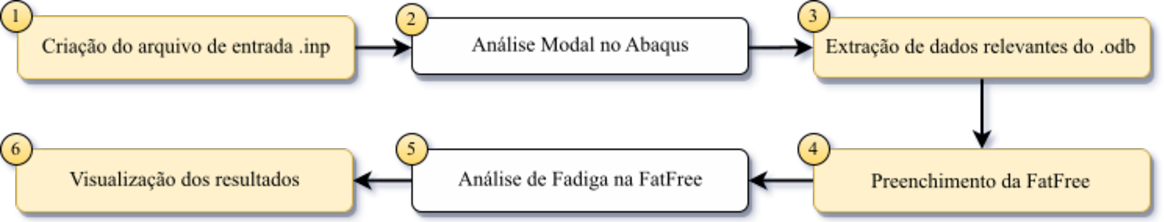
\includegraphics[width=\textwidth]{imagens/fluxograma_automatizado}
\end{figure}

De forma mais detalhada, a ferramente deve:

\begin{enumerate}[label= (\arabic*)]
    \item A partir de um arquivo de entrada com informações do modelo, criar arquivos de entrada para o ABAQUS (.inp) que reproduza todo o processo de simulação do comportamento do duto apresentado (\autoref{chap:assentamento}).
    \item Submeter o arquivo gerado para análise no ABAQUS.
    \item Processar os arquivos de saída do ABAQUS (.odb) extraindo os informações relevantes como a configuração deformada, modos de vibração, etc., gerando arquivos em outros formatos de fácil leitura para pós-processamento, tanto por este \textit{framework}, quanto por outro softwares.
    \item Pós-processar as informações gerando gráficos e relatórios relevantes para as tomadas de decisão do usuário quanto ao projeto. Esse é o requisito mais crítico, uma vez que é fundamental o entendimento sobre a análise de duto em vão-livre. Entre as tarefas que fazem parte deste item está a automação da escolha dos modos de vibração ativos e relevantes e para cada vão de interesse---a qual deve ser norteada pelos aspectos discutidos na \autoref{sec:multimode} --- e a manipulação da FatFree\footnote{Planilha Microsoft Office Excel desenvolvida pela \dnvf105 focada no cálculo de vida a fadiga de dutos submarinos.}.
    \item Ativar o processo de cálculo de fadiga no arquivo preenchido no passo anterior.
    \item Capturar os resultados arquivo, que agora contém os resultados do cálculo de vida a fadiga, e apresentá-los na forma de gráficos e relatórios.
\end{enumerate}

\section{Linguagem de programação}

Python\footnote{https://www.python.org} foi a linguagem de programação adotada. Além de ser uma linguagem interpretada de alto nível Orientada a Objeto --- que permite um alto índice de reaproveitamento de código --- e da sintaxe simples, \citeonline{rao2018} apresenta algumas das principais vantagens que destaca a linguagem para este tipo de aplicação:

\begin{itemize}
    \item Disponibilidade de bibliotecas para aplicações cientificas contemplando manipulação de matrizes (Numpy), funções matemáticas (SciPy), manipulação de dados em forma tabular (Pandas), criação de gráficos interativos (Matplotlib e Bokeh).

    \item Suporte para automação de tarefas. Os recursos de \textit{script} internos do Python e vários pacotes têm um forte suporte à automação de tarefas. A automação de tarefas repetitivas e a realização do registro de dados são fáceis e requerem pouco esforço. O ABAQUS, por exemplo, permite modelagem e acesso a informações em arquivos de saída via Python. A biblioteca xlwings permite manipulação planilhas Excel, a exemplo da FatFree.

    \item Pacotes Python como Django e Flask tornam possível desenvolver e usar o Python como uma API\footnote{Na programação de computadores, uma Interface de Programação de Aplicativos (\textit{Application Programming Interface}---API) é um conjunto de definições de sub-rotinas e ferramentas para a criação de software. Em termos gerais, é um conjunto de métodos de comunicação claramente definidos entre vários componentes.} com um \textit{front-end} da web. Essa funcionalidade é particularmente útil para reaproveitamento do \textit{framework}  em outras aplicações.
\end{itemize}

\section{Pacotes e classes}

Para implementação do fluxo de trabalho proposto para o \textit{framework}, prevê-se a implementação de módulos para lidar com cada contexto específico. Em python, módulos podem ser quaisquer arquivos com extensão \texttt{.py}. Estes módulos podem ser agrupados em pacotes, que são pastas que, além dos módulos, contém um arquivo \texttt{\_\_init\_\_.py}. No \textit{framework} têm-se os seguintes pacotes: % chktex 21

\begin{itemize}
    \item \texttt{model\_generator}: pacote principal responsável orquestrar o fluxo de trabalho do \textit{framework} desde o processamento dos dados de entrada, geração dos arquivos para o ABAQUS e os pós-processamentos.

    \item \texttt{odb\_handler}: responsável por lidar com os arquivos de saída do ABAQUS (odb) e guardar os dados relevantes em arquivos com formatos de fácil manipulação (CSV, JSON, etc\ldots).

    \item \texttt{mode\_selector}: pacote responsável pela estratégia de seleção automática de modos de vibração para cada vão e manipulação dos dados associados vãos e seus respectivos modos.

    \item \texttt{dnv}: pacote que implementa os cálculos dos modelos de resposta da \dnvf105 e manipula a planilha FatFree por meio da biblioteca xlwings.

    \item \texttt{plots}: pacote responsável pro agregar as funções de geração de gráficos dos resultados.
\end{itemize}

Já dentre as principais classes estão:

\begin{itemize}
    \item \texttt{Model}: classe que contém as informações do modelo do problema.
    A classe armazena todas as informações para construção dos arquivos \texttt{.inp}, isto é, dados de batimetria, material, geometria do duto, coeficientes de segurança, entre outros.
    A instanciação dessa classe deve ocorrer mediante o processamento de um arquivo principal de entrada com esses dados, em formato JSON (\autoref{apendice:json}).

    \item \texttt{Inp}: lida com a escrita modularizada de arquivos de entrada  para o ABAQUS. A proposta é que se crie um arquivo principal que terá inclusão de outros arquivos acessórios que terão as informações específicas de cada aspecto da modelagem: batimetria, passos de carga, etc.

    \item \texttt{Span}: classe que representa um vão do duto. Dentre os métodos da classe estão os métodos responsáveis pela seleção dos modos de vibração.

    \item \texttt{ModeShape}: classe que representa um mode de vibração (\textit{mode shape}).
\end{itemize}

A \autoref{fig:UML} exibe um diagrama UML com esses módulos e classes, suas relações de pertencimento e dependência, e os principais métodos e atributos das classes.

\begin{figure}[!ht]
    \centering
    \caption{Diagrama UML dos módulos e classes.}\label{fig:UML}
    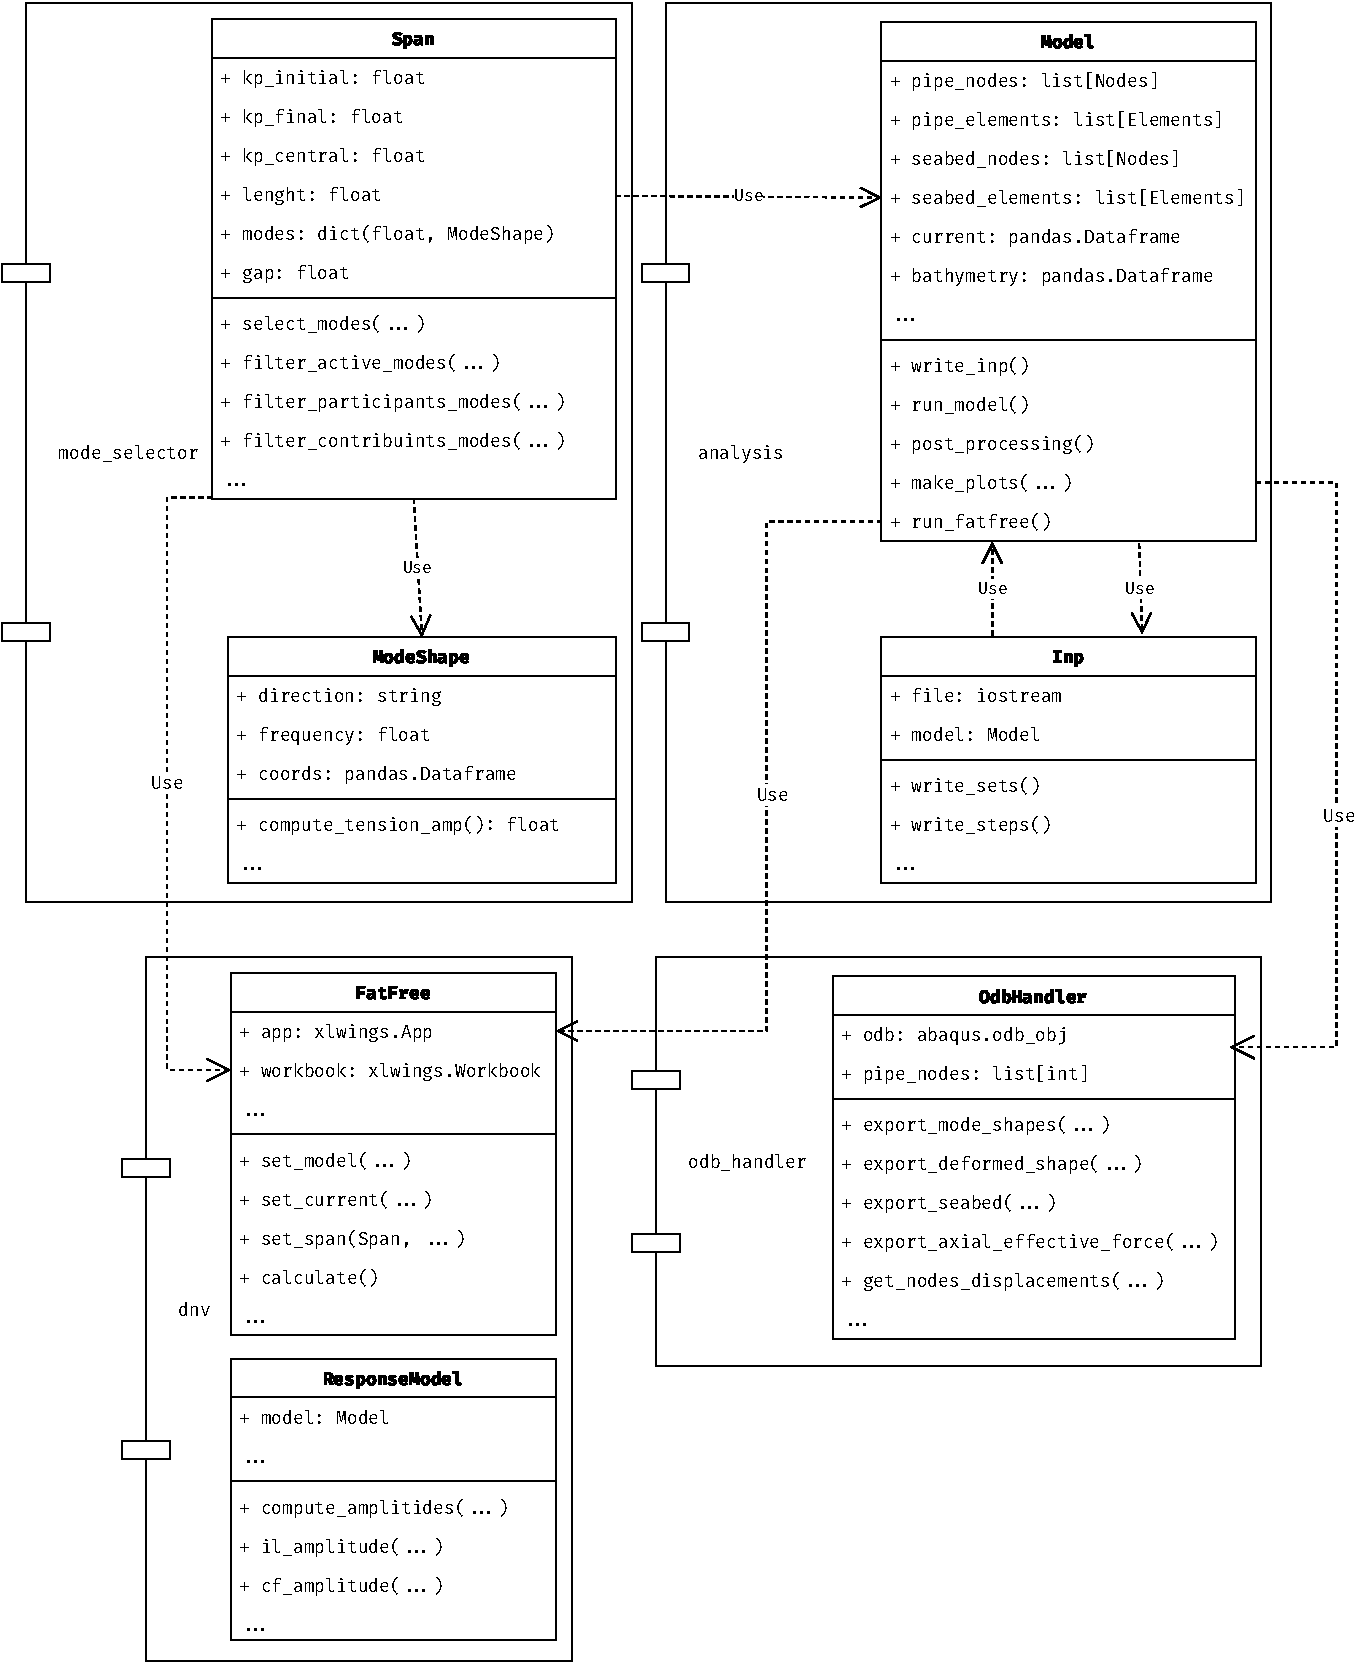
\includegraphics[width=0.95\textwidth]{imagens/UML}
    \fonte{Autor (2019)}
\end{figure}
